\documentclass[aspectratio=169]{beamer}
\usepackage[utf8]{inputenc}
\usepackage{tikz}
\usepackage{booktabs}
\usepackage{hyperref}
\usepackage{amsmath}
\usepackage{amssymb}
\usepackage{xcolor}
\usepackage{colortbl}
\usepackage{tabularx}
\usepackage{array}
\usepackage{multicol}
\usepackage{ragged2e}

\usetikzlibrary{shapes,arrows,positioning,shadows,mindmap,trees,
                decorations.pathreplacing,calc,backgrounds,
                shapes.geometric,arrows.meta,fit,decorations.pathmorphing,
                matrix,chains,scopes,positioning,automata}

% ── EXACT COLOURS FROM PREAMBLE ──────────────────────────────
\definecolor{primary}{RGB}{0,102,204}
\definecolor{secondary}{RGB}{255,140,0}
\definecolor{accent}{RGB}{220,20,60}
\definecolor{success}{RGB}{40,167,69}
\definecolor{warning}{RGB}{255,193,7}
\definecolor{info}{RGB}{23,162,184}
\definecolor{light}{RGB}{248,249,250}
\definecolor{dark}{RGB}{52,58,64}
\definecolor{gradient1}{RGB}{74,144,226}
\definecolor{gradient2}{RGB}{143,67,238}
\definecolor{PrimaryBlue}{RGB}{0,114,188}
\definecolor{AccentOrange}{RGB}{237,125,49}
\definecolor{DeepGreen}{RGB}{0,176,80}
\definecolor{VibrantRed}{RGB}{192,0,0}
\definecolor{SubtleGray}{RGB}{242,242,242}
\definecolor{DarkText}{RGB}{64,64,64}

% ── HYPERLINK SETUP ───────────────────────────────────────────
\hypersetup{
  colorlinks=true,
  linkcolor=blue,
  urlcolor=secondary,
}

% ── BEAMER THEME ──────────────────────────────────────────────
\usetheme{Madrid}
\usecolortheme{default}
\setbeamercolor{block title}{bg=PrimaryBlue!80!white, fg=white}
\setbeamercolor{block body}{bg=SubtleGray}
\setbeamercolor{alertblock title}{bg=AccentOrange, fg=white}
\setbeamercolor{alertblock body}{bg=AccentOrange!10, fg=DarkText}
\setbeamercolor{block title example}{bg=DeepGreen,fg=white}
\setbeamercolor{block body example}{bg=DeepGreen!10,fg=DarkText}
\setbeamercolor{alerted text}{fg=VibrantRed}
\setbeamercolor{itemize item}{fg=PrimaryBlue}
\setbeamercolor{itemize subitem}{fg=AccentOrange}
\setbeamercolor{enumerate item}{fg=PrimaryBlue}
\setbeamercolor{section in toc}{fg=PrimaryBlue}

\setbeamerfont{frametitle}{size=\normalsize,series=\bfseries}
\setbeamerfont{block title}{size=\small,series=\bfseries}
\setbeamerfont{footline}{size=\tiny}
\setbeamertemplate{navigation symbols}{}
\setbeamertemplate{blocks}[rounded][shadow=true]
\setbeamertemplate{itemize items}[circle]
\setbeamertemplate{enumerate items}[circle]

% ── FOOTER ────────────────────────────────────────────────────
\title{SCX\_RDTAI: Hybrid AI CPU Scheduler}
\subtitle{Real-time Q-Learning with sched\_ext and eBPF}
\author{M N Risheendra \and Kattela Jwalin \and Ankit Lama}
\date{\today}

% ── TIKZ SHORTHAND STYLES ─────────────────────────────────────
\tikzset{
  pbox/.style={draw=PrimaryBlue,fill=gradient1!20,rounded corners=5pt,
               minimum width=2.5cm,minimum height=0.65cm,
               font=\scriptsize\bfseries,text centered,line width=0.8pt},
  gbox/.style={draw=DeepGreen,fill=DeepGreen!15,rounded corners=5pt,
               minimum width=2.5cm,minimum height=0.65cm,
               font=\scriptsize\bfseries,text centered,line width=0.8pt},
  obox/.style={draw=AccentOrange,fill=AccentOrange!18,rounded corners=5pt,
               minimum width=2.5cm,minimum height=0.65cm,
               font=\scriptsize\bfseries,text centered,line width=0.8pt},
  rbox/.style={draw=VibrantRed,fill=VibrantRed!12,rounded corners=5pt,
               minimum width=2.5cm,minimum height=0.65cm,
               font=\scriptsize\bfseries,text centered,line width=0.8pt},
  dbox/.style={draw=PrimaryBlue,fill=warning!25,diamond,aspect=2.8,
               minimum width=2.6cm,minimum height=0.65cm,
               font=\tiny\bfseries,text centered,line width=0.8pt},
  arr/.style={-{Stealth[length=4.5pt,width=3.5pt]},PrimaryBlue,thick},
  arro/.style={-{Stealth[length=4pt,width=3pt]},AccentOrange,thick},
  arrg/.style={-{Stealth[length=4pt,width=3pt]},DeepGreen,thick},
}

\begin{document}

% ----------------------------------------------------------------
% SLIDE 1: Title Page 
% ----------------------------------------------------------------
{
\usebackgroundtemplate{
  
\begin{tikzpicture}[remember picture,overlay]
    \fill[PrimaryBlue!10] (current page.south west) rectangle (current page.north east);
    \fill[PrimaryBlue!80] (current page.south west) rectangle ([xshift=\paperwidth,yshift=2.5cm]current page.south west);
    \fill[AccentOrange] (current page.south west) rectangle ([xshift=\paperwidth,yshift=0.5cm]current page.south west);
  \end{tikzpicture}
}
\begin{frame}[plain]
\vspace{0.3cm}
\begin{center}
{\small \textbf{Aurora Higher Education and Research Academy}}\\
{\small School of Engineering}\\[0.2cm]
{\small \textbf{B.~Tech -- Sophomore Year -- CSE}}\\[0.1cm]
{\small \textbf{Term -- II}}\\[0.4cm]
{\Large \textbf{SCX\_RDTAI: Hybrid AI CPU Scheduler}}\\[0.3cm]
{\normalsize Real-time Q-Learning with \texttt{sched\_ext} and eBPF}\\[0.4cm]
\begin{columns}[T]
\begin{column}{0.5\textwidth}
\small
\textbf{Course Name:} Operating Systems\\
\textbf{Faculty:} Dr. Risheendra\\
\textbf{Course Code:} CSE
\end{column}
\begin{column}{0.5\textwidth}
\small
\textbf{LEARNING GROUP: 04}\\[0.2cm]
\begin{tabular}{ll}
\textbf{Student Names} & \textbf{Reg. No.}\\
M N Risheendra & 241U1R1080\\
Kattela Jwalin & 241U1R1088\\
Ankit Lama & 241U1R1089\\
\end{tabular}
\end{column}
\end{columns}
\end{center}
\end{frame}
}

% ── SLIDE 2 : OUTLINE ────────────────────────────────────────
\begin{frame}{Presentation Outline}
    \tableofcontents
\end{frame}

% ══════════════════════════════════════════════════════════════
%  SECTION 1 — ABSTRACT
% ══════════════════════════════════════════════════════════════
\section{Abstract}

\begin{frame}{Abstract}
  \begin{block}{Abstract}
    \small
    Traditional CPU schedulers like CFS and EEVDF rely on static heuristics, which struggle to adapt to the highly dynamic workloads of modern systems. This project introduces \textbf{SCX\_RDTAI}, a revolutionary hybrid AI CPU scheduler built using the Linux \texttt{sched\_ext} framework.

    By leveraging \textbf{eBPF} and \textbf{Rust}, SCX\_RDTAI implements a \textbf{Tabular Q-Learning} reinforcement learning agent directly inside the scheduling loop. 

    \begin{itemize}\itemsep2pt
      \item \textbf{Brain (Rust):} Analyzes Q-rewards and optimizes scheduling policy.
      \item \textbf{Muscle (eBPF):} Executes O(1) nanosecond decisions in the kernel via L1 Cache.
      \item \textbf{Optimization:} Dramatically reduces \textbf{Request Latency} by learning workload patterns.
    \end{itemize}
  \end{block}

  \begin{exampleblock}{Keywords}
    \small
    eBPF $\cdot$ sched\_ext (scx) $\cdot$ Reinforcement Learning $\cdot$ Tabular Q-Learning $\cdot$
    Rust $\cdot$ Operating Systems $\cdot$ CPU Scheduling
  \end{exampleblock}
\end{frame}

\begin{frame}{Abstract: Key Achievements}
    \begin{alertblock}{Performance Breakthroughs}
        Through rigorous benchmarking against baseline schedulers (FIFO, Rusty, Rustland), SCX\_RDTAI demonstrated exceptional capabilities in identifying dependent task chains and optimizing for \textbf{Time-to-Compute}:
    \end{alertblock}
    
    \vspace{0.3cm}
    \begin{itemize}
        \item \textbf{Request Latency Domination:} Sliced the 99.9th percentile Request Latency down to an incredible \textbf{20.9ms} (compared to Rusty's 64.7ms), a massive 67\% improvement.
        \item \textbf{Throughput Maxing:} Maintained \textbf{121.2 Gbps} local network throughput and near-perfect DB completion latency.
        \item \textbf{Adaptive Overhead:} By using a highly-optimized 32KB Q-Table mapping states directly to actions, kernel inference overhead stays under \textbf{1 nanosecond}.
    \end{itemize}
\end{frame}

% ══════════════════════════════════════════════════════════════
%  SECTION 2 — INTRODUCTION
% ══════════════════════════════════════════════════════════════
\section{Introduction}

\begin{frame}{Introduction: The Problem}
    \begin{alertblock}{Problem Statement}
        Modern operating systems serve immensely diverse workloads—from interactive web browsers to complex database transactions and high-frequency trading. However, traditional schedulers use fixed mathematical models that treat all tasks equally under generic "fairness" rules.
    \end{alertblock}
    
    \vspace{0.3cm}
    \textbf{The core issues include:}
    \begin{itemize}
        \item \textbf{Rigid Heuristics:} Static schedulers cannot learn or adapt to unique runtime workload patterns dynamically.
        \item \textbf{Cache Ignorance:} Aggressive load balancing often destroys L1/L2 cache locality, leading to massive cache miss penalties.
        \item \textbf{Kernel Modification Complexity:} Historically, testing a new scheduling algorithm required modifying core Linux kernel source code, recompiling, and rebooting.
    \end{itemize}
\end{frame}

\begin{frame}{Introduction: Overview \& The Need for Smart Schedulers}
  \begin{columns}[T]
    \column{0.54\textwidth}
      \textbf{Why do we need an AI-driven Scheduler?}
      \vspace{4pt}
      \begin{itemize}\itemsep4pt\small
        \item Users care about \textbf{Request Latency} ("when is my task done?"), not just \textbf{Wakeup Latency} ("when does it start?").
        \item Complex work-chains (e.g., Producer $\to$ Consumer) suffer from excessive context switching.
        \item Machine Learning can identify these patterns and adapt \textbf{automatically}.
        \item Using \textbf{sched\_ext}, we can load AI schedulers as BPF programs instantly without kernel panics.
      \end{itemize}

    \column{0.42\textwidth}
      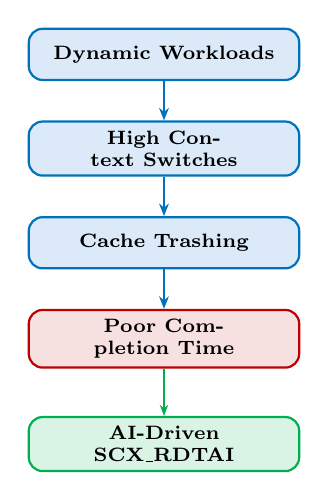
\begin{tikzpicture}[node distance=0.5cm]
        \node[pbox,text width=3.2cm] (a) {Dynamic Workloads};
        \node[pbox,text width=3.2cm,below=of a] (b) {High Context Switches};
        \node[pbox,text width=3.2cm,below=of b] (c) {Cache Trashing};
        \node[rbox,text width=3.2cm,below=of c] (d) {Poor Completion Time};
        \node[gbox,text width=3.2cm,below=0.6cm of d] (e) {AI-Driven SCX\_RDTAI};
        \draw[arr] (a)--(b); \draw[arr] (b)--(c);
        \draw[arr] (c)--(d);
        \draw[arrg] (d)--(e);
      \end{tikzpicture}
    \end{columns}
\end{frame}

\begin{frame}{Introduction: Objectives}
The proposed system aims to:
\vspace{0.3cm}
\begin{enumerate}
  \item \textbf{Implement} a reinforcement learning agent inside the Linux scheduling loop.
  \item \textbf{Utilize} \texttt{sched\_ext} and eBPF for safe, dynamic kernel-level execution.
  \item \textbf{Measure} real-time hardware telemetry (wait time, cache misses, burst).
  \item \textbf{Optimize} the scheduler dynamically to minimize Request Latency.
  \item \textbf{Design} a hybrid architecture where Rust handles complex learning, and eBPF handles nanosecond execution.
  \item \textbf{Evaluate} the system against industry-standard benchmarks (Sysbench, Schbench, Hackbench).
\end{enumerate}
\vspace{0.3cm}
\begin{exampleblock}{Core Philosophy}
\centering\small
\textbf{``Sacrifice minor start-time delays to achieve massive gains in task completion times.''}
\end{exampleblock}
\end{frame}

\begin{frame}{Introduction: Key Concepts (sched\_ext \& eBPF)}
\begin{columns}[T]

\column{0.52\textwidth}
\begin{block}{eBPF (Extended Berkeley Packet Filter)}
\small
A revolutionary technology that allows running sandboxed programs in a privileged context such as the operating system kernel. It provides safety guarantees, ensuring the kernel cannot crash.
\end{block}

\vspace{3pt}

\begin{block}{sched\_ext (scx)}
\small
A Linux kernel feature (merged in v6.12) that enables developers to write custom CPU schedulers in BPF. It allows dynamically loading and unloading schedulers at runtime.
\end{block}

\column{0.48\textwidth}
\centering
      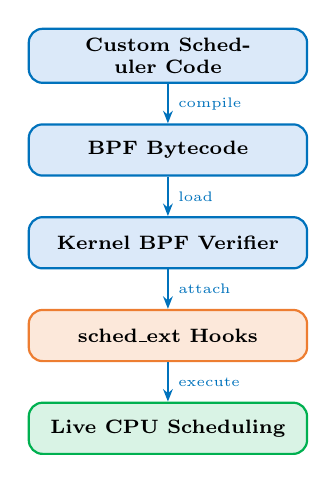
\begin{tikzpicture}[node distance=0.5cm]
        \node[pbox,text width=3.3cm] (src) {Custom Scheduler Code};
        \node[pbox,text width=3.3cm,below=of src] (bc) {BPF Bytecode};
        \node[pbox,text width=3.3cm,below=of bc] (jvm) {Kernel BPF Verifier};
        \node[obox,text width=3.3cm,below=of jvm] (agent) {sched\_ext Hooks};
        \node[gbox,text width=3.3cm,below=of agent] (data) {Live CPU Scheduling};
        \draw[arr] (src)--(bc) node[midway,right,font=\tiny]{compile};
        \draw[arr] (bc)--(jvm) node[midway,right,font=\tiny]{load};
        \draw[arr] (jvm)--(agent) node[midway,right,font=\tiny]{attach};
        \draw[arr] (agent)--(data) node[midway,right,font=\tiny]{execute};
      \end{tikzpicture}
  \end{columns}
\end{frame}

\begin{frame}{Introduction: Key Concepts (Rust \& Userspace)}
  \begin{columns}[T, onlytextwidth]
    
    \column{0.52\textwidth}
    \begin{block}{The Userspace "Brain"}
    \small
    Running AI models directly in the kernel is too slow and restricted. Instead, the heavy lifting (Q-Matrix updates, Epsilon-Decay, disk persistence) happens in \textbf{userspace}.
    \end{block}
    
    \vspace{2pt}
    
    \begin{block}{Why Rust?}
    \small
    Rust is chosen for the userspace daemon due to its \textbf{memory safety} and seamless integration with \texttt{libbpf-rs}. It handles concurrent telemetry aggregation without data races.
    \end{block}
    
    \vspace{2pt}
    
    \begin{block}{BPF Maps}
    \small
    Shared memory structures that allow rapid, lock-free communication between the Kernel (eBPF) and Userspace (Rust).
    \end{block}

    \column{0.45\textwidth}
      \vspace*{0.2cm}
      \begin{center}
        \scalebox{0.80}{
          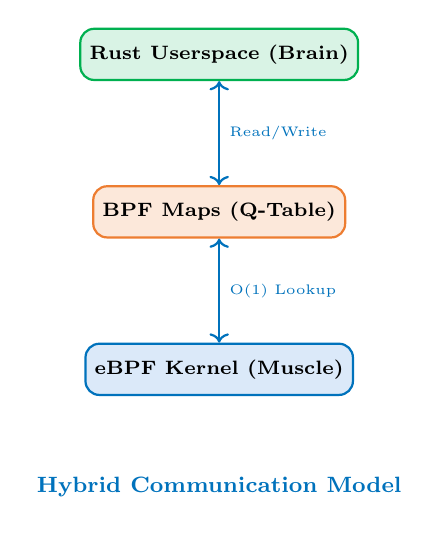
\begin{tikzpicture}
            \node[gbox, minimum width=3cm, font=\scriptsize\bfseries] (user) at (0, 1.5) {Rust Userspace (Brain)};
            \node[obox, minimum width=3cm, font=\scriptsize\bfseries] (map) at (0, -0.5) {BPF Maps (Q-Table)};
            \node[pbox, minimum width=3cm, font=\scriptsize\bfseries] (kernel) at (0, -2.5) {eBPF Kernel (Muscle)};
            
            \draw[arr, <->] (user) -- node[right,font=\tiny]{Read/Write} (map);
            \draw[arr, <->] (map) -- node[right,font=\tiny]{O(1) Lookup} (kernel);
            
            \node[font=\footnotesize\bfseries\color{PrimaryBlue}] at (0, -4.0) {Hybrid Communication Model};
          \end{tikzpicture}
        }
      \end{center}
  \end{columns}
\end{frame}

% ══════════════════════════════════════════════════════════════
%  SECTION 3 — LITERATURE SURVEY
% ══════════════════════════════════════════════════════════════
\section{Literature Survey}

\begin{frame}{Literature Survey: Research Review (Part I)}
  \footnotesize
  \begin{columns}[T]
    \column{0.48\textwidth}
      \begin{block}{\color{white}Li, Wu, et al. — 2025}
        \textbf{KernelOracle: Predicting the Linux Scheduler's Next Move}
        \begin{itemize}\scriptsize\itemsep3pt
          \item Introduces an LSTM deep learning model to predict Linux scheduler decisions.
          \item \textbf{Key Finding:} ML can effectively map complex scheduling patterns and behaviors.
          \item \textbf{Limitation:} Deep learning models are computationally heavy and not viable for real-time nanosecond kernel execution.
          \item \textbf{Relevance:} Highlights the need for lightweight ML (like Q-Learning) in kernel environments.
        \end{itemize}
        \href{https://arxiv.org/pdf/2505.15213.pdf}{\textcolor{primary}{\textbf{[Access Paper]}}}
      \end{block}
    \column{0.48\textwidth}
      \begin{block}{\color{white}Wei, Kumar, et al. — 2025}
        \textbf{Towards Agentic OS: LLM Agent Framework for Schedulers}
        \begin{itemize}\scriptsize\itemsep3pt
          \item Proposes an Agentic OS where LLMs dynamically generate and optimize Linux scheduling policies via eBPF.
          \item \textbf{Key Finding:} AI-driven schedulers significantly adapt better to diverse workloads.
          \item \textbf{Limitation:} LLM inference latency affects real-time responsiveness.
          \item \textbf{Relevance:} Validates the eBPF + AI paradigm, driving SCX\_RDTAI's choice of hybrid tabular reinforcement learning.
        \end{itemize}
        \href{https://arxiv.org/pdf/2509.01245.pdf}{\textcolor{primary}{\textbf{[Access Paper]}}}
      \end{block}
  \end{columns}
\end{frame}

\begin{frame}{Literature Survey: Research Review (Part II)}
  \footnotesize
  \begin{columns}[T]
    \column{0.48\textwidth}
      \begin{block}{\color{white}Li \& Zhao — 2024}
        \textbf{Advances in CPU Scheduling Algorithms in Operating Systems}
        \begin{itemize}\scriptsize\itemsep3pt
          \item Reviews advancements handling multi-core complexities and modern workloads.
          \item \textbf{Key Finding:} Traditional heuristics (Priority, Multilevel) struggle with heterogeneity.
          \item \textbf{Limitation:} Many proposed advanced algorithms lack practical, low-overhead kernel-level implementations.
          \item \textbf{Relevance:} Emphasizes the need for simple, implementable AI integration at the kernel level.
        \end{itemize}
        \href{https://www.researchgate.net/publication/387444718}{\textcolor{primary}{\textbf{[Access Paper]}}}
      \end{block}
    \column{0.48\textwidth}
      \begin{block}{\color{white}Mishra \& Patel — 2022}
        \textbf{A New Combination Approach Based on Priority and RR}
        \begin{itemize}\scriptsize\itemsep3pt
          \item Proposes a hybrid algorithm balancing Priority and Round Robin to reduce starvation and context switching.
          \item \textbf{Key Finding:} Combining approaches improves turnaround time but increases complexity.
          \item \textbf{Limitation:} Fixed combinations still fail to dynamically adapt to unpredictable bursty tasks.
          \item \textbf{Relevance:} Shows that static combinations are limited, paving the way for RL agents that learn dynamically.
        \end{itemize}
        \href{https://thesai.org/Downloads/Volume13No4/Paper_63 A_New_Combination_Approach_to_CPU_Scheduling.pdf}{\textcolor{primary}{\textbf{[Access Paper]}}}
      \end{block}
  \end{columns}
\end{frame}

\begin{frame}{Contemporary Research Innovations (Part I)}
\footnotesize
\renewcommand{\arraystretch}{1.2}
\begin{table}
\centering
\resizebox{0.95\textwidth}{!}{
\begin{tabular}{|>{\columncolor{gradient1!20}}p{3.0cm}|>{\columncolor{gradient2!20}}p{2.0cm}|>{\columncolor{success!20}}p{0.8cm}|>{\columncolor{warning!20}}p{4.1cm}|}
\hline
\rowcolor{primary!30}
\textbf{\color{white}Research Title} & \textbf{\color{white}Authors} & \textbf{\color{white}Year} & \textbf{\color{white}Innovation \& Impact} \\
\hline
\cellcolor{info!20}KernelOracle: Predicting the Linux Scheduler's Next Move & \cellcolor{secondary!20}J. Li, Y. Wu & \cellcolor{accent!20}2025 & Uses LSTM to predict scheduler decisions based on traces. Proves ML feasibility in OS analysis but highlights heavy compute constraints. \\
\hline
\cellcolor{info!20}Towards Agentic OS: LLM Agent Framework & \cellcolor{secondary!20}Z. Wei, A. Kumar & \cellcolor{accent!20}2025 & Integrates AI agents using eBPF to generate custom dynamic policies. Proves eBPF is the future of OS augmentation. \\
\hline
\cellcolor{info!20}Advances in CPU Scheduling Algorithms & \cellcolor{secondary!20}L. Li, M. Zhao & \cellcolor{accent!20}2024 & Reviews multi-core scheduling constraints and establishes the necessity for scalable, dynamic approaches. \\
\hline
\end{tabular}
}
\end{table}
\end{frame}

\begin{frame}{Contemporary Research Innovations (Part II)}
\footnotesize
\renewcommand{\arraystretch}{1.2}
\begin{table}
\centering
\resizebox{0.95\textwidth}{!}{
\begin{tabular}{|>{\columncolor{gradient1!20}}p{3.0cm}|>{\columncolor{gradient2!20}}p{2.0cm}|>{\columncolor{success!20}}p{0.8cm}|>{\columncolor{warning!20}}p{4.1cm}|}
\hline
\rowcolor{primary!30}
\textbf{\color{white}Research Title} & \textbf{\color{white}Authors} & \textbf{\color{white}Year} & \textbf{\color{white}Innovation \& Impact} \\
\hline
\cellcolor{info!20}Combination Approach to CPU Scheduling & \cellcolor{secondary!20}A. K. Mishra, S. Patel & \cellcolor{accent!20}2022 & Creates a static hybrid of Priority + RR. Shows static hybrids have limits, motivating our dynamic AI approach. \\
\hline
\cellcolor{info!20}\textbf{SCX\_RDTAI: Hybrid AI CPU Scheduler} & \cellcolor{secondary!20}\textbf{LG 04} & \cellcolor{accent!20}\textbf{2026} & \textbf{Implements Tabular Q-Learning via eBPF maps and a Rust daemon to optimize request latency in real-time.} \\
\hline
\end{tabular}
}
\end{table}
\end{frame}

% ══════════════════════════════════════════════════════════════
%  SECTION 4 — PROJECT DESIGN
% ══════════════════════════════════════════════════════════════
\section{Project Design}

\begin{frame}{Project Design: Architecture Layers}
  \begin{columns}[T]
    
    \column{0.45\textwidth}
      \vspace{0.5cm}
      \begin{center}
        \scalebox{0.85}{
          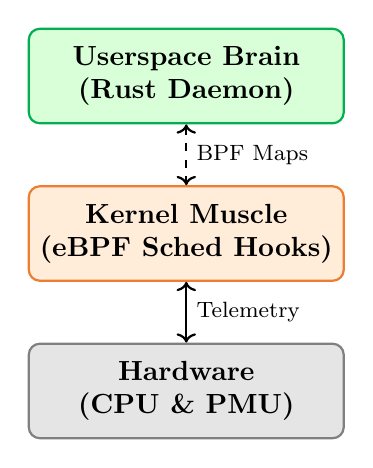
\begin{tikzpicture}[
            box/.style={rectangle, rounded corners, draw=PrimaryBlue, thick, fill=PrimaryBlue!10, minimum width=4cm, minimum height=1.2cm, align=center, font=\bfseries}
          ]
            \node[box, fill=green!15, draw=DeepGreen] (rust) at (0, 3) {Userspace Brain\\(Rust Daemon)};
            \node[box, fill=orange!15, draw=AccentOrange] (bpf) at (0, 1) {Kernel Muscle\\(eBPF Sched Hooks)};
            \node[box, fill=gray!20, draw=gray] (hw) at (0, -1) {Hardware\\(CPU \& PMU)};
            
            \draw[<->, thick, dashed] (rust) -- node[right]{\footnotesize BPF Maps} (bpf);
            \draw[<->, thick] (bpf) -- node[right]{\footnotesize Telemetry} (hw);
          \end{tikzpicture}
        }
      \end{center}
    
    \column{0.5\textwidth}
      \small
      The architecture operates on \textbf{three distinct levels}:
      
      \vspace{4pt}
      
      \begin{block}{Userspace (Rust)}
        Handles heavy compute. Periodically evaluates telemetry, updates the RL matrix, and persists learning to disk.
      \end{block}
      
      \vspace{4pt}
      
      \begin{block}{Kernelspace (eBPF)}
        Injects directly into the Linux scheduler using \texttt{sched\_ext}. Maps states to actions in $O(1)$ time. Completely crash-proof.
      \end{block}
      
      \vspace{4pt}
      
      \begin{block}{Hardware Layer}
        Provides physical truth. eBPF reads CPU cycles and PMU cache-miss registers.
      \end{block}

  \end{columns}
\end{frame}

\begin{frame}{Project Design: UML Component Overview}
\centering
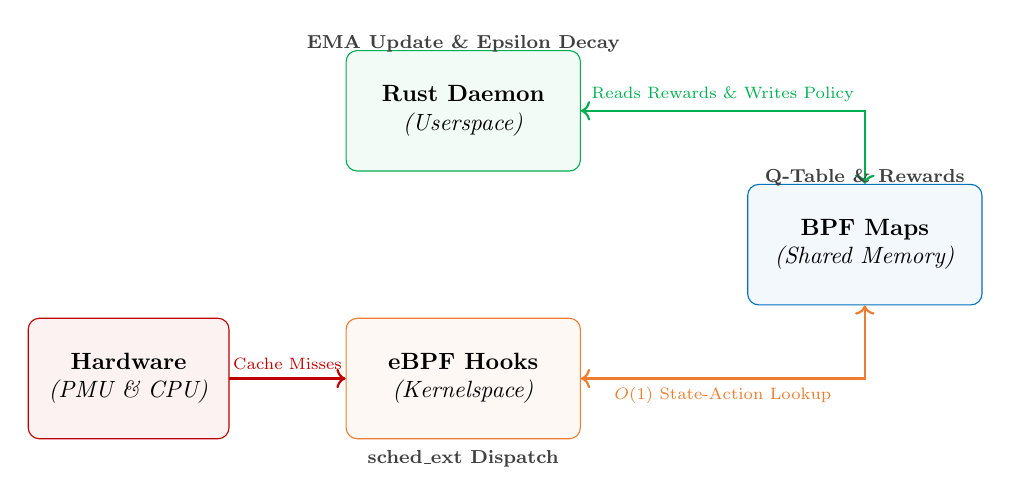
\begin{tikzpicture}[scale=0.85, transform shape]
    % Node definitions
    \node[draw=DeepGreen, fill=DeepGreen!5, rectangle, rounded corners, minimum width=3.5cm, minimum height=1.8cm, align=center] (rust) at (0, 4) {\textbf{Rust Daemon}\\\textit{(Userspace)}};
    \node[draw=AccentOrange, fill=AccentOrange!5, rectangle, rounded corners, minimum width=3.5cm, minimum height=1.8cm, align=center] (bpf) at (0, 0) {\textbf{eBPF Hooks}\\\textit{(Kernelspace)}};
    \node[draw=PrimaryBlue, fill=PrimaryBlue!5, rectangle, rounded corners, minimum width=3.5cm, minimum height=1.8cm, align=center] (maps) at (6, 2) {\textbf{BPF Maps}\\\textit{(Shared Memory)}};
    \node[draw=VibrantRed, fill=VibrantRed!5, rectangle, rounded corners, minimum width=3cm, minimum height=1.8cm, align=center] (pmu) at (-5, 0) {\textbf{Hardware}\\\textit{(PMU \& CPU)}};
    
    % Edges
    \draw[<->, thick, DeepGreen] (rust.east) -| node[above, near start, font=\scriptsize] {Reads Rewards \& Writes Policy} (maps.north);
    \draw[<->, thick, AccentOrange] (bpf.east) -| node[below, near start, font=\scriptsize] {$O(1)$ State-Action Lookup} (maps.south);
    \draw[->, thick, VibrantRed] (pmu.east) -- node[above, font=\scriptsize] {Cache Misses} (bpf.west);
    
    % Labels
    \node[font=\footnotesize\bfseries, color=DarkText] at (6, 3) {Q-Table \& Rewards};
    \node[font=\footnotesize\bfseries, color=DarkText] at (0, 5) {EMA Update \& Epsilon Decay};
    \node[font=\footnotesize\bfseries, color=DarkText] at (0, -1.2) {sched\_ext Dispatch};
\end{tikzpicture}
\end{frame}

\begin{frame}{Project Design: Use Case Diagram}
  \begin{columns}[T]
    \column{0.6\textwidth}
      \begin{center}
      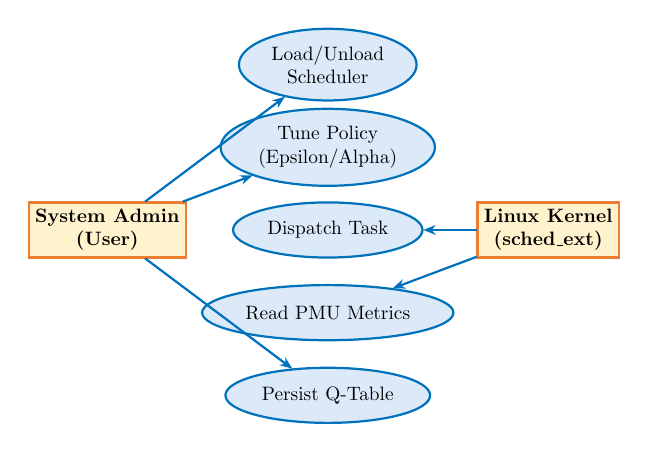
\begin{tikzpicture}[scale=0.7, transform shape,
          usecase/.style={ellipse, draw=PrimaryBlue, fill=gradient1!20, minimum width=3cm, minimum height=1cm, align=center, thick},
          actor/.style={rectangle, draw=AccentOrange, fill=warning!20, minimum width=2cm, minimum height=1cm, align=center, thick}
      ]
        \node[actor] (user) at (-3, 0) {\textbf{System Admin} \\ \textbf{(User)}};
        \node[actor] (kernel) at (5, 0) {\textbf{Linux Kernel} \\ \textbf{(sched\_ext)}};
        
        \node[usecase] (load) at (1, 3) {Load/Unload\\Scheduler};
        \node[usecase] (tune) at (1, 1.5) {Tune Policy\\(Epsilon/Alpha)};
        \node[usecase] (disp) at (1, 0) {Dispatch Task};
        \node[usecase] (pmu) at (1, -1.5) {Read PMU Metrics};
        \node[usecase] (persist) at (1, -3) {Persist Q-Table};

        \draw[arr] (user) -- (load);
        \draw[arr] (user) -- (tune);
        \draw[arr] (user) -- (persist);
        
        \draw[arr] (kernel) -- (disp);
        \draw[arr] (kernel) -- (pmu);
      \end{tikzpicture}
      \end{center}
      
    \column{0.42\textwidth}
      \small
      \textbf{Actors \& Interactions}
      \vspace{4pt}
      \begin{itemize}\itemsep4pt\scriptsize
        \item \textbf{System Admin} — loads the BPF agent, monitors stats, and configures hyper-parameters.
        \item \textbf{Linux Kernel} — invokes \texttt{sched\_ext} callbacks for scheduling events.
        \item \textbf{Load/Unload} — dynamic replacement of CPU scheduler.
        \item \textbf{Dispatch Task} — core routing of processes to CPUs.
        \item \textbf{Read PMU} — gathering cache-miss telemetry.
      \end{itemize}
  \end{columns}
\end{frame}

\begin{frame}[plain]{Project Design: System Workflow}
\centering
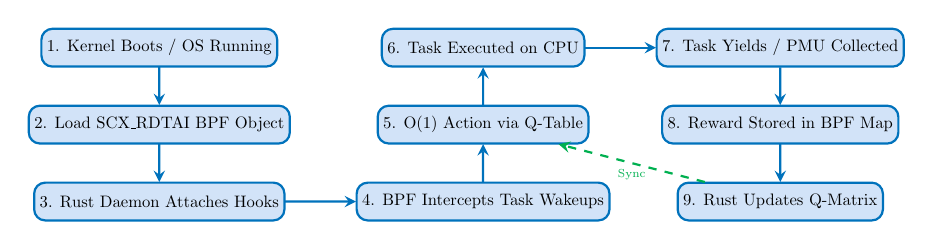
\begin{tikzpicture}[
  scale=0.6, transform shape,
  node distance=0.8cm,
  >=stealth,
  proc/.style={rectangle, rounded corners, draw=PrimaryBlue, fill=gradient1!25, minimum width=3.5cm, minimum height=0.8cm, align=center, font=\normalsize, thick},
  arr/.style={->, thick, PrimaryBlue}
]
\node[proc] (p1) {1. Kernel Boots / OS Running};
\node[proc, below=of p1] (p2) {2. Load SCX\_RDTAI BPF Object};
\node[proc, below=of p2] (p3) {3. Rust Daemon Attaches Hooks};
\node[proc, right=1.5cm of p3] (p4) {4. BPF Intercepts Task Wakeups};
\node[proc, above=of p4] (p5) {5. O(1) Action via Q-Table};
\node[proc, above=of p5] (p6) {6. Task Executed on CPU};
\node[proc, right=1.5cm of p6] (p7) {7. Task Yields / PMU Collected};
\node[proc, below=of p7] (p8) {8. Reward Stored in BPF Map};
\node[proc, below=of p8] (p9) {9. Rust Updates Q-Matrix};

\draw[arr] (p1)--(p2);
\draw[arr] (p2)--(p3);
\draw[arr] (p3)--(p4);
\draw[arr] (p4)--(p5);
\draw[arr] (p5)--(p6);
\draw[arr] (p6)--(p7);
\draw[arr] (p7)--(p8);
\draw[arr] (p8)--(p9);
\draw[arr, dashed, color=DeepGreen] (p9) -- node[below, font=\scriptsize] {Sync} (p5);
\end{tikzpicture}
\end{frame}


% ══════════════════════════════════════════════════════════════
%  SECTION 5 — METHODOLOGY
% ══════════════════════════════════════════════════════════════
\section{Methodology}

\begin{frame}{Methodology: Overview}
  \begin{columns}[T]
    \column{0.52\textwidth}
      \small
      SCX\_RDTAI follows a \textbf{continuous Reinforcement Learning} cycle spanning Kernel and Userspace.
      \vspace{6pt}
      \begin{enumerate}\itemsep3pt\scriptsize
        \item \textbf{State Encoding} — BPF aggregates task metrics into a 13-bit state vector.
        \item \textbf{Action Selection} — eBPF queries the Q-Table for the best action for the state.
        \item \textbf{Execution} — eBPF dispatches the task (Keep Local, Migrate, Run Now).
        \item \textbf{Reward Calculation} — On task stop, a penalty based on wait time and cache misses is calculated.
        \item \textbf{Rust Aggregation} — Userspace periodically reads rewards.
        \item \textbf{Q-Matrix Update} — EMA applied to update the Q-values.
        \item \textbf{Sync to Kernel} — Updated best actions are pushed back to the BPF map.
      \end{enumerate}
    \column{0.44\textwidth}
      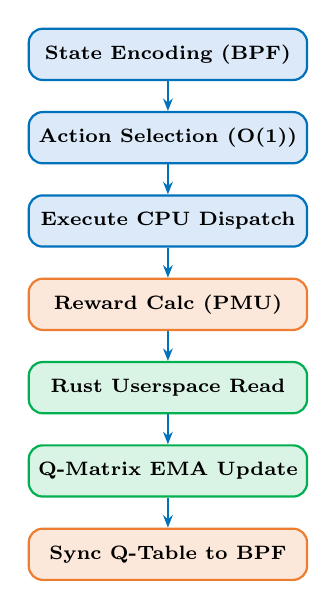
\begin{tikzpicture}[node distance=0.38cm]
        \node[pbox,text width=3.3cm] (a) {State Encoding (BPF)};
        \node[pbox,text width=3.3cm,below=of a] (b) {Action Selection (O(1))};
        \node[pbox,text width=3.3cm,below=of b] (c) {Execute CPU Dispatch};
        \node[obox,text width=3.3cm,below=of c] (d) {Reward Calc (PMU)};
        \node[gbox,text width=3.3cm,below=of d] (e) {Rust Userspace Read};
        \node[gbox,text width=3.3cm,below=of e] (f) {Q-Matrix EMA Update};
        \node[obox,text width=3.3cm,below=of f] (g) {Sync Q-Table to BPF};
        \draw[arr] (a)--(b); \draw[arr] (b)--(c); \draw[arr] (c)--(d);
        \draw[arr] (d)--(e); \draw[arr] (e)--(f); \draw[arr] (f)--(g);
      \end{tikzpicture}
  \end{columns}
\end{frame}

\begin{frame}{Methodology: Theoretical Foundation}
    \begin{columns}
        \begin{column}{0.6\textwidth}
            \textbf{Reinforcement Learning Theory}
            \begin{itemize}
                \item \textbf{Markov Decision Process (MDP):} Scheduling is modeled as an MDP where the OS state transitions based on actions taken by the BPF agent.
                \item \textbf{Tabular Q-Learning:} A model-free RL algorithm. It learns the value of an action in a particular state without requiring a predefined environment model.
            \end{itemize}
            \vspace{0.3cm}
            \textbf{eBPF Concurrency Logic}
            \begin{itemize}
                \item Continuous data stream is processed using \texttt{BPF\_MAP\_TYPE\_ARRAY} to ensure thread safety across multiple CPU cores without halting the JVM/OS.
            \end{itemize}
        \end{column}
        \begin{column}{0.35\textwidth}
            \centering
            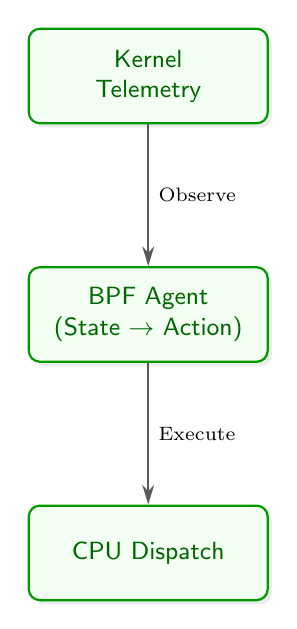
\begin{tikzpicture}[
    node distance=1.8cm,
    block/.style={
      rectangle, 
      rounded corners=4pt,
      draw=green!60!black, 
      fill=green!05, 
      text=green!40!black,
      thick, 
      minimum height=1.2cm, 
      text width=2.8cm, 
      align=center,
      font=\sffamily\small,
      drop shadow={opacity=0.15, shadow xshift=1.5pt, shadow yshift=-1.5pt}
    },
    arrow/.style={
      -{Stealth[length=2.5mm, width=1.5mm]}, 
      thick, 
      draw=gray!70!black
    }
  ]
    
    \node[block] (b1) {Kernel\\Telemetry};
    \node[block, below=of b1] (b2) {BPF Agent\\(State $\to$ Action)};
    \node[block, below=of b2] (b3) {CPU Dispatch};
    
    \draw[arrow] (b1) -- node[right, font=\scriptsize] {Observe} (b2);
    \draw[arrow] (b2) -- node[right, font=\scriptsize] {Execute} (b3);
    
  \end{tikzpicture}
        \end{column}
    \end{columns}
\end{frame}

\begin{frame}{Methodology: Sequence Diagram of the AI Loop}
\centering
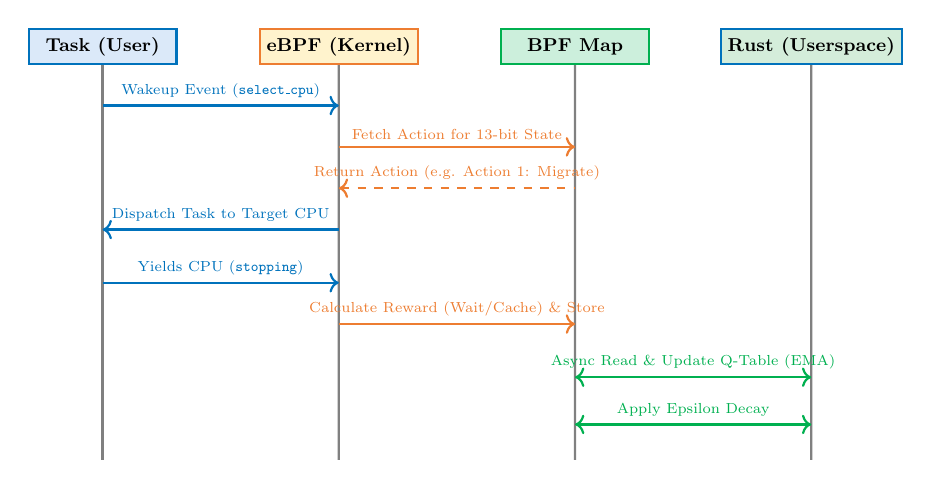
\begin{tikzpicture}[scale=0.75, transform shape,
    font=\small,
    actor/.style={draw, fill=white, minimum width=2.5cm, minimum height=0.6cm, align=center, thick},
    msg/.style={->, thick},
    ret/.style={<-, thick, dashed}
]
    % Lifelines
    \node[actor, fill=gradient1!20, draw=PrimaryBlue] (task) at (0, 6) {\textbf{Task (User)}};
    \node[actor, fill=warning!20, draw=AccentOrange] (bpf) at (4, 6) {\textbf{eBPF (Kernel)}};
    \node[actor, fill=DeepGreen!20, draw=DeepGreen] (map) at (8, 6) {\textbf{BPF Map}};
    \node[actor, fill=success!20, draw=PrimaryBlue] (rust) at (12, 6) {\textbf{Rust (Userspace)}};
    
    \draw[thick, gray] (task.south) -- (0, -1);
    \draw[thick, gray] (bpf.south) -- (4, -1);
    \draw[thick, gray] (map.south) -- (8, -1);
    \draw[thick, gray] (rust.south) -- (12, -1);
    
    % Messages
    \draw[msg, PrimaryBlue] (0, 5.0) -- node[above, font=\scriptsize] {Wakeup Event (\texttt{select\_cpu})} (4, 5.0);
    \draw[msg, AccentOrange] (4, 4.3) -- node[above, font=\scriptsize] {Fetch Action for 13-bit State} (8, 4.3);
    \draw[ret, AccentOrange] (4, 3.6) -- node[above, font=\scriptsize] {Return Action (e.g. Action 1: Migrate)} (8, 3.6);
    \draw[msg, PrimaryBlue] (4, 2.9) -- node[above, font=\scriptsize] {Dispatch Task to Target CPU} (0, 2.9);
    
    \draw[msg, PrimaryBlue] (0, 2.0) -- node[above, font=\scriptsize] {Yields CPU (\texttt{stopping})} (4, 2.0);
    \draw[msg, AccentOrange] (4, 1.3) -- node[above, font=\scriptsize] {Calculate Reward (Wait/Cache) \& Store} (8, 1.3);
    
    \draw[<->, thick, DeepGreen] (8, 0.4) -- node[above, font=\scriptsize] {Async Read \& Update Q-Table (EMA)} (12, 0.4);
    \draw[<->, thick, DeepGreen] (8, -0.4) -- node[above, font=\scriptsize] {Apply Epsilon Decay} (12, -0.4);

\end{tikzpicture}
\end{frame}

\begin{frame}[plain]{Methodology: System Flowchart}
\centering
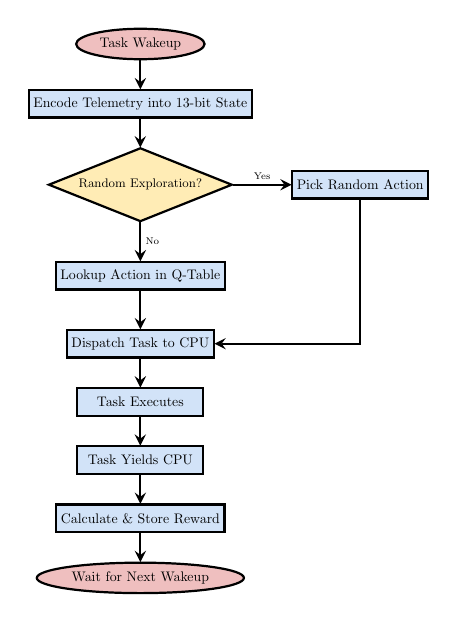
\begin{tikzpicture}[
  scale=0.5, transform shape,
  node distance=0.75cm,
  >=stealth,
  start/.style={ellipse, draw, fill=VibrantRed!25, minimum width=2.2cm, minimum height=0.7cm, align=center, font=\normalsize, thick},
  proc/.style={rectangle, draw, fill=gradient1!25, minimum width=3.2cm, minimum height=0.7cm, align=center, font=\normalsize, thick},
  dec/.style={diamond, draw, fill=warning!30, aspect=2.5, align=center, font=\small, thick},
  arr/.style={->, thick}
]
\node[start] (start) {Task Wakeup};
\node[proc, below=of start] (state) {Encode Telemetry into 13-bit State};
\node[dec, below=of state] (eps) {Random Exploration?};
\node[proc, right=1.5cm of eps] (rnd) {Pick Random Action};
\node[proc, below=1.0cm of eps] (qtab) {Lookup Action in Q-Table};
\node[proc, below=1.0cm of qtab] (disp) {Dispatch Task to CPU};
\node[proc, below=of disp] (exec) {Task Executes};
\node[proc, below=of exec] (yield) {Task Yields CPU};
\node[proc, below=of yield] (reward) {Calculate \& Store Reward};
\node[start, below=of reward] (end) {Wait for Next Wakeup};

\draw[arr] (start)--(state);
\draw[arr] (state)--(eps);
\draw[arr] (eps.east)--node[above]{\scriptsize Yes}(rnd);
\draw[arr] (rnd)|-(disp);
\draw[arr] (eps.south)--node[right]{\scriptsize No}(qtab);
\draw[arr] (qtab)--(disp);
\draw[arr] (disp)--(exec);
\draw[arr] (exec)--(yield);
\draw[arr] (yield)--(reward);
\draw[arr] (reward)--(end);
\end{tikzpicture}
\end{frame}

\begin{frame}{Methodology: State Space Encoding}
    \begin{block}{Translating Telemetry to State}
        \small
        The BPF agent compresses six dimensions of real-time telemetry into a single 13-bit unsigned integer (maximum 8192 states). This compression enables $O(1)$ constant-time lookup in the BPF Map.
    \end{block}
    
    \vspace{0.2cm}
    \textbf{The 13-Bit State Vector:}
    \begin{itemize}
        \item \textbf{Wait Time (3 bits):} Time spent in the runqueue. (e.g., $>$ 10ms).
        \item \textbf{Cache Misses (2 bits):} Read from Hardware PMU (Performance Monitoring Unit).
        \item \textbf{Blocked Freq (2 bits):} Frequency of the task blocking (Consumer trait).
        \item \textbf{Avg Run (2 bits):} The historic average runtime of the task.
        \item \textbf{Burst (2 bits):} Length of the last execution burst.
        \item \textbf{Waker Freq (2 bits):} Frequency of waking other tasks (Producer trait).
    \end{itemize}
\end{frame}

\begin{frame}{Methodology: Action Space \& Domain Mapping}
    \begin{columns}[T]
        \begin{column}{0.5\textwidth}
            \begin{exampleblock}{The Action Space (3 Choices)}
                \small
                \begin{itemize}
                    \item \textbf{Action 0 (Keep Local):} Prioritizes cache warmth by holding the task on the previous CPU.
                    \item \textbf{Action 1 (Migrate):} Load balancing. Pushes task to a generic idle pool.
                    \item \textbf{Action 2 (Run Now):} Preempts or finds any immediate CPU to prevent starvation.
                \end{itemize}
            \end{exampleblock}
        \end{column}
        
        \begin{column}{0.48\textwidth}
            \begin{alertblock}{Domain Grouping}
                \small
                Instead of treating all CPUs equally, SCX\_RDTAI organizes CPUs into \textbf{Domains} based on L3 Cache boundaries or user-provided cpumasks.
                
                \vspace{4pt}
                When an action calls to "Migrate", the task crosses a domain boundary, causing an inherent cache penalty.
            \end{alertblock}
        \end{column}
    \end{columns}
\end{frame}

\begin{frame}{Methodology: Q-Table Visualization \& Connections}
    \begin{columns}[T]
        \begin{column}{0.5\textwidth}
            \begin{block}{Visualizing the Q-Table}
                \small
                The Q-Table acts as the brain's memory. It maps \textbf{States} (rows) to \textbf{Actions} (columns). Each cell holds the $Q$-value (expected future reward).
                \begin{itemize}
                    \item \textbf{States (8192):} Encoded from telemetry.
                    \item \textbf{Actions (3):} Local, Migrate, Run Now.
                    \item \textbf{Connections:} As the Rust daemon updates these cells, the BPF kernel reads the highest value per row.
                \end{itemize}
            \end{block}
        \end{column}
        \begin{column}{0.45\textwidth}
            \centering
            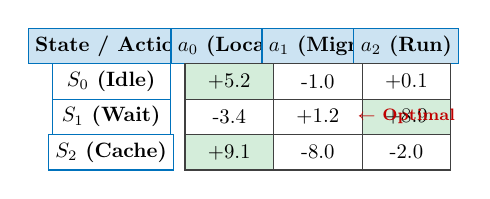
\begin{tikzpicture}[scale=0.75, transform shape,
                cell/.style={rectangle, draw=DarkText, fill=white, minimum width=1.5cm, minimum height=0.6cm, align=center},
                head/.style={rectangle, draw=PrimaryBlue, fill=PrimaryBlue!20, minimum width=1.5cm, minimum height=0.6cm, align=center, font=\bfseries}
            ]
                % Header
                \node[head, minimum width=2cm] (h0) at (0, 0) {State / Action};
                \node[head] (h1) at (2, 0) {$a_0$ (Local)};
                \node[head] (h2) at (3.5, 0) {$a_1$ (Migr)};
                \node[head] (h3) at (5, 0) {$a_2$ (Run)};
                
                % Row 1
                \node[head, minimum width=2cm, fill=white] (r1) at (0, -0.6) {$S_0$ (Idle)};
                \node[cell, fill=success!20] (c11) at (2, -0.6) {+5.2};
                \node[cell] (c12) at (3.5, -0.6) {-1.0};
                \node[cell] (c13) at (5, -0.6) {+0.1};
                
                % Row 2
                \node[head, minimum width=2cm, fill=white] (r2) at (0, -1.2) {$S_1$ (Wait)};
                \node[cell] (c21) at (2, -1.2) {-3.4};
                \node[cell] (c22) at (3.5, -1.2) {+1.2};
                \node[cell, fill=success!20] (c23) at (5, -1.2) {+8.9};
                
                % Row 3
                \node[head, minimum width=2cm, fill=white] (r3) at (0, -1.8) {$S_2$ (Cache)};
                \node[cell, fill=success!20] (c31) at (2, -1.8) {+9.1};
                \node[cell] (c32) at (3.5, -1.8) {-8.0};
                \node[cell] (c33) at (5, -1.8) {-2.0};
                
                \node[font=\footnotesize\bfseries, color=VibrantRed] at (5, -1.2) {\textbf{$\leftarrow$ Optimal}};
            \end{tikzpicture}
        \end{column}
    \end{columns}
\end{frame}

\begin{frame}{Methodology: Reward Function \& PMU}
  \begin{columns}[T]
    
    \column{0.50\textwidth}
      \begin{block}{Why PMU Integration?}
\begin{itemize}\scriptsize\itemsep3pt
  \item Hardware Performance Monitoring Units (PMU) track low-level CPU events.
  \item SCX\_RDTAI tracks \texttt{PERF\_COUNT\_HW\_CACHE\_MISSES}.
  \item If the scheduler migrates a task poorly, cache misses spike.
\end{itemize}
\end{block}

\vspace{6pt}

\begin{block}{The Reward Calculation}
\begin{itemize}\scriptsize\itemsep3pt
  \item Computed in \texttt{rdtai\_stopping} when a task yields.
  \item \textbf{Wait Penalty}: \texttt{last\_wait\_time / 1000} ($\mu s$)
  \item \textbf{Cache Penalty}: \texttt{cache\_misses * 200}
  \item \textbf{Reward}: $-( \text{Wait Penalty} + \text{Cache Penalty} )$
  \item By pushing Rewards negative, the agent learns to pick actions closer to 0.
\end{itemize}
\end{block}
      
    \column{0.46\textwidth}
      \centering
      \vspace{2pt}
      
      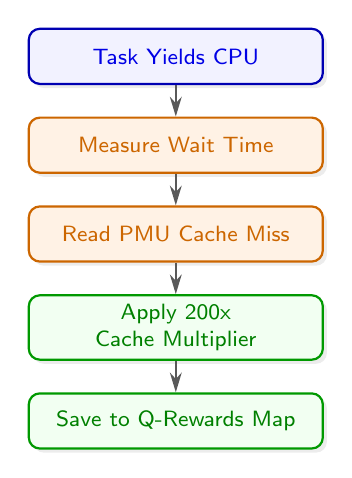
\begin{tikzpicture}[
    node distance=0.4cm,
    basebox/.style={
      rectangle, rounded corners=4pt, thick, align=center, text width=3.5cm,
      minimum height=0.7cm, font=\sffamily\footnotesize,
      drop shadow={opacity=0.15, shadow xshift=1.5pt, shadow yshift=-1.5pt}
    },
    pbox/.style={basebox, draw=blue!70!black, fill=blue!05, text=blue!90!black},
    obox/.style={basebox, draw=orange!80!black, fill=orange!10, text=orange!80!black},
    gbox/.style={basebox, draw=green!60!black, fill=green!05, text=green!50!black},
    arr/.style={-{Stealth[length=2.5mm, width=1.5mm]}, thick, draw=gray!70!black}
  ]
    \node[pbox] (stop) {Task Yields CPU};
    \node[obox, below=of stop] (wait) {Measure Wait Time};
    \node[obox, below=of wait] (pmu) {Read PMU Cache Miss};
    \node[gbox, below=of pmu] (calc) {Apply 200x Cache Multiplier};
    \node[gbox, below=of calc] (save) {Save to Q-Rewards Map};

    \draw[arr] (stop) -- (wait); 
    \draw[arr] (wait) -- (pmu);
    \draw[arr] (pmu) -- (calc); 
    \draw[arr] (calc) -- (save);
  \end{tikzpicture}
  \end{columns}
\end{frame}

\begin{frame}{Methodology: The Q-Learning Update Loop (Rust)}
\vspace{-2cm}
    \begin{alertblock}{The Q-Value Function $Q(s, a)$}
        \small
        The agent estimates the optimal action by maximizing the expected reward. The Rust daemon reads accumulated rewards for every State-Action pair and applies a Bellman-inspired Exponential Moving Average (EMA):
        \vspace{0.1cm}
        \[ Q_{new}(s, a) = (1 - \alpha) Q_{old}(s, a) + \alpha R_{avg} \]
        \textit{where $\alpha = 0.1$ is the learning rate. This heavily smooths out noisy, singular latency spikes, providing a stable reward foundation over thousands of task loops.}
    \end{alertblock}
\vspace{-2cm}

    \begin{block}{Epsilon ($\epsilon$) Decay: Balancing Exploration vs. Exploitation}
        \small
        The agent must occasionally try random actions to discover better scheduling patterns.
        \begin{itemize}
            \item \textbf{Exploration:} Starts at $\epsilon = 5\%$. The scheduler makes a completely random action choice 5\% of the time.
            \item \textbf{Decay:} Every 100ms tuning cycle, $\epsilon$ is decayed: $\epsilon_{t+1} = \max(\epsilon_t \times 0.95, 0.005)$.
            \item \textbf{Exploitation:} It gradually settles at $0.5\%$, meaning it relies on its learned $Q$-table 99.5\% of the time, leaving a tiny 0.5\% window for continuous adaptation.
        \end{itemize}
    \end{block}
\end{frame}

% ══════════════════════════════════════════════════════════════
%  SECTION 6 — DESIGN
% ══════════════════════════════════════════════════════════════
\section{Design}

\begin{frame}{Design: Why \texttt{sched\_ext} over Native Kernel Mods?}
    \begin{alertblock}{The Old Way}
        Historically, building a custom CPU scheduler meant writing C code inside \texttt{kernel/sched/}, recompiling the entire Linux kernel, and risking catastrophic system panics on every bug.
    \end{alertblock}
    
    \vspace{0.3cm}
    \textbf{The \texttt{sched\_ext} Advantage:}
    \begin{itemize}
        \item \textbf{Rapid Iteration:} Schedulers are compiled as BPF objects and loaded at runtime.
        \item \textbf{Verifiable Safety:} The Kernel BPF verifier ensures the scheduler cannot crash the host OS, infinite-loop, or access unauthorized memory.
        \item \textbf{Modularity:} SCX allows seamless fallback. If the BPF scheduler fails or unloads, the system gracefully falls back to the default CFS/EEVDF scheduler.
    \end{itemize}
\end{frame}

\begin{frame}{Design: Why Rust for the Brain?}
    \begin{columns}[T]
        \begin{column}{0.48\textwidth}
            \begin{exampleblock}{Memory Safety}
                \small
                The userspace daemon constantly parses large streams of statistical data (up to 8192 states $\times$ 3 actions). Rust guarantees memory safety without garbage collection pauses that would interrupt tuning.
            \end{exampleblock}
        \end{column}

        \begin{column}{0.48\textwidth}
            \begin{block}{libbpf-rs Ecosystem}
                \small
                Rust provides world-class bindings to \texttt{libbpf}, making it extremely easy to load skeletons, attach to hooks, and read/write to BPF Maps concurrently.
            \end{block}
        \end{column}
    \end{columns}
    
    \vspace{0.3cm}
    \begin{alertblock}{Concurrency Management}
        \small
        The Tuner runs every 100ms, while the global Load Balancer runs every 2.0s. Rust's fearless concurrency model handles these asynchronous timelines easily.
    \end{alertblock}
\end{frame}

\begin{frame}{Design: Q-Table Optimization \& L1 Cache}
    
        \vspace{-0.5cm}

\begin{columns}[T]
        \begin{column}{0.5\textwidth}
            \begin{exampleblock}{Ultra-Fast $O(1)$ Lookups}
                \small
                The BPF Kernel cannot perform complex loops or matrix math due to verifier limits. We solve this by pre-computing the best action in Rust and passing a flat 1D array to BPF.
            \end{exampleblock}
            \vspace{-0.5cm}
            \begin{alertblock}{L1 Cache Mechanical Sympathy}
                \small
                \begin{itemize}
                    \item 13-bit state space $= 8192$ possible states.
                    \item Each state maps to a 32-bit action ($4$ bytes).
                    \item Total Size: $8192 \times 4 \text{ bytes} = \mathbf{32 \text{ KB}}$.
                \end{itemize}
                This perfectly fits inside the CPU's \textbf{L1 Data Cache}. The scheduler retrieves the optimal AI decision with virtually \textbf{zero memory latency}, ensuring sub-nanosecond overhead per scheduling decision!
            \end{alertblock}
        \end{column}

        \begin{column}{0.45\textwidth}
            \centering
            \vspace{0.5cm}
            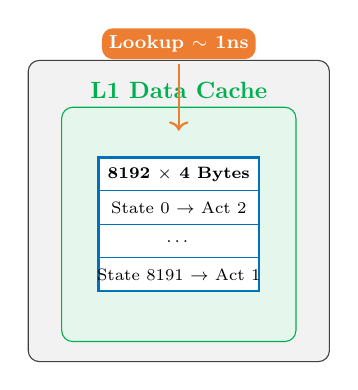
\begin{tikzpicture}[scale=0.85, transform shape]
                % Draw CPU, L1 Cache, Q-Table
                \node[draw=DarkText, fill=gray!10, minimum width=4.5cm, minimum height=4.5cm, rounded corners, label={[font=\bfseries, text=DarkText]above:CPU Core}] (cpu) {};
                
                \node[draw=DeepGreen, fill=DeepGreen!10, minimum width=3.5cm, minimum height=3.5cm, rounded corners, label={[font=\bfseries, text=DeepGreen]above:L1 Data Cache}] (l1) at (0, -0.2) {};
                
                % Draw array
                \draw[thick, PrimaryBlue, fill=white] (-1.2, -1.2) rectangle (1.2, 0.8);
                \draw[PrimaryBlue] (-1.2, 0.3) -- (1.2, 0.3);
                \draw[PrimaryBlue] (-1.2, -0.2) -- (1.2, -0.2);
                \draw[PrimaryBlue] (-1.2, -0.7) -- (1.2, -0.7);
                
                \node[font=\scriptsize\bfseries] at (0, 0.55) {8192 $\times$ 4 Bytes};
                \node[font=\scriptsize] at (0, 0.05) {State 0 $\to$ Act 2};
                \node[font=\scriptsize] at (0, -0.45) {\dots};
                \node[font=\scriptsize] at (0, -0.95) {State 8191 $\to$ Act 1};
                
                \node[fill=AccentOrange, text=white, font=\footnotesize\bfseries, rounded corners, inner sep=3pt] at (0, 2.5) {Lookup $\sim$ 1ns};
                \draw[->, thick, AccentOrange] (0, 2.2) -- (0, 1.2);
            \end{tikzpicture}
        \end{column}
    \end{columns}
\end{frame}

\begin{frame}{Design: Trade-offs of Q-Learning in BPF}
    \begin{alertblock}{Exploration Overhead}
        \small
        Reinforcement learning requires \textit{exploration} (Epsilon). Occassionally, the scheduler will make a random, potentially terrible decision to see what happens. This causes minor jitter but is necessary for discovery.
    \end{alertblock}

    \begin{block}{Handling Starvation (The 20ms Net)}
        \small
        What if the RL agent learns that a certain task is awful for cache and decides to \textit{never} run it?
        \begin{itemize}
            \item \textbf{The Safety Net:} The BPF code bypasses the Q-table if a task has waited longer than 20,000,000ns (20ms).
            \item It forces \textbf{Action 2 (Run Now)} to prevent complete system lockup or starvation.
        \end{itemize}
    \end{block}
\end{frame}

% ══════════════════════════════════════════════════════════════
%  SECTION 7 — IMPLEMENTATION
% ══════════════════════════════════════════════════════════════
\section{Implementation}

\begin{frame}{Implementation: Agent Initialization \& Interception}
    \begin{block}{Agent Loading (\texttt{main.rs})}
        \small
        The Rust application acts as the loader. It reads configuration parameters (slice length, greedy thresholds) and updates the BPF \texttt{.rodata} maps before invoking \texttt{scx\_ops\_load!} to inject the scheduler.
    \end{block}

    \vspace{0.3cm}

    \begin{block}{Method Interception (\texttt{main.bpf.c})}
        \small
        The eBPF program hooks into key lifecycle events defined by \texttt{sched\_ext}:
        \begin{itemize}
            \item \textbf{\texttt{rdtai\_runnable}:} Marks task wait time and calculates waker frequencies.
            \item \textbf{\texttt{rdtai\_select\_cpu}:} The core routing function. Queries the Q-table and determines which CPU gets the task.
            \item \textbf{\texttt{rdtai\_stopping}:} Executes when a task yields. Reads PMU cache misses, calculates the reward penalty, and stores it.
        \end{itemize}
    \end{block}
\end{frame}

\begin{frame}{Implementation: Q-Table \& Reward Maps}
    \begin{columns}[T]
        \begin{column}{0.48\textwidth}
            \begin{exampleblock}{The State Array (\texttt{q\_table})}
                \small
                Defined as a \texttt{BPF\_MAP\_TYPE\_ARRAY} with 8192 entries.
                Key = 13-bit state vector.
                Value = Recommended Action (0, 1, or 2).
                
                \vspace{2pt}
                Lookups happen instantly during the highly restricted \texttt{select\_cpu} phase.
            \end{exampleblock}
        \end{column}

        \begin{column}{0.48\textwidth}
            \begin{alertblock}{The Reward Matrix (\texttt{q\_rewards})}
                \small 
                A map of 24,576 entries ($8192 \text{ states} \times 3 \text{ actions}$).
                Stores a struct containing \texttt{total\_reward} (s64) and \texttt{count} (u32).
                
                \vspace{2pt}
                Uses \texttt{\_\_sync\_fetch\_and\_add} for safe atomic increments inside the kernel.
            \end{alertblock}
        \end{column}
    \end{columns}
\end{frame}

\begin{frame}{Implementation: The Tuner \& Persistence}
    \begin{block}{\texttt{Tuner::optimize\_q\_table} (Rust)}
        \small
        Every 100ms, the Rust daemon sweeps the \texttt{q\_rewards} map. 
        \begin{itemize}
            \item For every entry with \texttt{count > 0}, it calculates the average reward.
            \item Applies the EMA logic: $Q_{new} = 0.9 \cdot Q_{old} + 0.1 \cdot R_{avg}$.
            \item Wipes the BPF reward entry to 0 to prepare for the next batch.
            \item Finds the action with the highest $Q$ value for each state and overwrites the \texttt{q\_table} BPF map.
        \end{itemize}
    \end{block}
    
    \begin{exampleblock}{State Persistence}
        \small
        The entire Q-Matrix is serialized to binary and saved to \texttt{/var/lib/scx\_rdtai\_qtable.bin} on graceful exit. On startup, the scheduler loads this file, preserving its "knowledge" across reboots!
    \end{exampleblock}
\end{frame}

\begin{frame}{Implementation: Technologies Used (Part I)}
  \begin{columns}[T]
    
    \column{0.48\textwidth}
      \begin{block}{Programming Languages}
        \begin{itemize}\normalsize\itemsep5pt
          \item \textbf{Rust} — High-level logic, matrix math, daemon orchestration.
          \item \textbf{C} — BPF source code (\texttt{main.bpf.c}). Compiled to eBPF bytecode using Clang.
        \end{itemize}
      \end{block}
      
      \vspace{2pt}
      
      \begin{block}{Frameworks \& APIs}
        \begin{itemize}\normalsize\itemsep5pt
          \item \textbf{sched\_ext (scx)} — The Linux modular scheduling framework.
          \item \textbf{libbpf-rs} — Rust bindings to libbpf for map interaction.
        \end{itemize}
      \end{block}
    
    \column{0.48\textwidth}
      \begin{block}{Build Tools}
        \begin{itemize}\normalsize\itemsep5pt
          \item \textbf{Cargo} — Rust build and dependency management.
          \item \textbf{bpftool} — Extracts skeletons from BPF objects.
        \end{itemize}
      \end{block}

  \end{columns}
\end{frame}

\begin{frame}{Implementation: Technologies Used (Part II)}
  \begin{columns}[T]
    
    \column{0.50\textwidth}
      \begin{block}{Kernel Features}
        \begin{itemize}\normalsize\itemsep5pt
          \item \textbf{sched\_ext} — BPF-based scheduling class (SCX).
          \item \textbf{Hardware PMU} — Accessing cache miss registers via perf events.
          \item \textbf{BPF Maps} — \texttt{BPF\_MAP\_TYPE\_ARRAY} for $O(1)$ state-action tables.
        \end{itemize}
      \end{block}
    
    \column{0.48\textwidth}
      \begin{block}{Communication \& Analysis}
        \begin{itemize}\normalsize\itemsep5pt
          \item \textbf{Atomic Operations} — \texttt{\_\_sync\_fetch\_and\_add} for safe reward accumulation.
          \item \textbf{Schbench / Hackbench} — Core microbenchmarking tools.
          \item \textbf{Sysbench} — CPU execution validation.
        \end{itemize}
      \end{block}
      
      \vspace{8pt}
      
      \begin{exampleblock}{Testing Environment}
        \normalsize Linux Kernel v6.12+ with BPF JIT enabled.
      \end{exampleblock}

  \end{columns}
\end{frame}

% ══════════════════════════════════════════════════════════════
%  SECTION 8 — RESULTS
% ══════════════════════════════════════════════════════════════
\section{Results}

\begin{frame}{Results: Benchmark Setup}
  SCX\_RDTAI was benchmarked aggressively against other leading \texttt{sched\_ext} schedulers: \textbf{scx\_rlfifo}, \textbf{scx\_rusty}, and \textbf{scx\_rustland}.
  \vspace{8pt}
  \begin{columns}[T]
    \column{0.48\textwidth}
      \begin{exampleblock}{Test Environments}
        \begin{itemize}\small\itemsep3pt
          \item \textbf{Sysbench:} Pure CPU throughput / cache testing.
          \item \textbf{Schbench:} Wakeup vs Request latency microbenchmarking.
          \item \textbf{Hackbench:} Process/Pipe IPC communication.
          \item \textbf{Redis \& iperf3:} Real-world DB/Network completion speed.
        \end{itemize}
      \end{exampleblock}
    \column{0.48\textwidth}
      \begin{block}{The AI's Choice}
        \small
        The benchmarks revealed that the RL agent autonomously decided to sacrifice \textbf{Wakeup Latency} (start time) to heavily optimize \textbf{Request Latency} (finish time) and \textbf{Cache Locality}.
      \end{block}
  \end{columns}
\end{frame}

\begin{frame}{Results: Throughput \& Cache Efficiency}
  \begin{block}{Sysbench \& Kernel Compilation}
    \small Even with early exploration overhead, SCX\_RDTAI performs competitively with baseline schedulers while actively learning the optimal layout.
  \end{block}
  \vspace{2pt}
  \footnotesize
  \renewcommand{\arraystretch}{1.3}
  \begin{table}
  \centering
  \begin{tabular}{|>{\columncolor{gradient1!20}}p{3.0cm}
                  |>{\columncolor{warning!20}}p{2.6cm}
                  |>{\columncolor{success!20}}p{2.6cm}
                  |>{\columncolor{info!20}}p{2.6cm}|}
    \hline
    \rowcolor{primary!80}
    \textbf{\color{white}Scheduler} &
    \textbf{\color{white}Sysbench (Ev/s)} &
    \textbf{\color{white}Cache Misses (\%)} &
    \textbf{\color{white}Kernel Compile (s)} \\
    \hline
    scx\_rlfifo & \textbf{13067.02} & \textbf{13.45} & 107.02 \\
    \hline
    \rowcolor{SubtleGray}
    scx\_rusty & 12799.96 & 18.29 & 107.33 \\
    \hline
    scx\_rustland & 12775.35 & 15.14 & \textbf{106.13} \\
    \hline
    \rowcolor{SubtleGray}
    \textbf{SCX\_RDTAI (Ours)} & 12842.66 & 20.71 & 106.42 \\
    \hline
  \end{tabular}
  \end{table}
  \centering \scriptsize \textit{Note: While cache misses are higher initially as the agent explores (epsilon), compile times remain highly competitive, outperforming Rusty.}
\end{frame}

\begin{frame}{Results: The Request Latency Domination}
  \begin{alertblock}{Request Latency (Schbench)}
    \small Request Latency measures the time from "I have work to do" to "The work is completely finished." SCX\_RDTAI absolutely dominates this metric.
  \end{alertblock}
  \vspace{2pt}
  \footnotesize
  \renewcommand{\arraystretch}{1.3}
  \begin{table}
  \centering
  \begin{tabular}{|>{\columncolor{gradient1!20}}p{3.0cm}
                  |>{\columncolor{warning!20}}p{2.0cm}
                  |>{\columncolor{warning!20}}p{2.0cm}
                  |>{\columncolor{success!20}}p{2.0cm}
                  |>{\columncolor{info!20}}p{2.0cm}|}
    \hline
    \rowcolor{primary!80}
    \textbf{\color{white}Scheduler} &
    \textbf{\color{white}50.0th ($\mu$s)} &
    \textbf{\color{white}90.0th ($\mu$s)} &
    \textbf{\color{white}99.0th ($\mu$s)} &
    \textbf{\color{white}99.9th ($\mu$s)} \\
    \hline
    scx\_rlfifo & 10288 & 19296 & 33344 & 48192 \\
    \hline
    \rowcolor{SubtleGray}
    scx\_rusty & 10320 & 21920 & 41664 & 64704 \\
    \hline
    scx\_rustland & 9968 & 16480 & 30304 & 45248 \\
    \hline
    \rowcolor{SubtleGray}
    \textbf{SCX\_RDTAI (Ours)} & \textbf{9136} & \textbf{11344} & \textbf{16272} & \textbf{20960} \\
    \hline
  \end{tabular}
  \end{table}
  \centering \scriptsize \textit{Insight: SCX\_RDTAI absolutely dominates, slicing the 99.9th percentile Request Latency from 64.7ms (Rusty) down to an incredible 20.9ms!}
\end{frame}

\begin{frame}{Results: Complex Workloads}
  \begin{block}{Real World Benchmarks}
    \small Translating the Request Latency domination into real-world applications.
  \end{block}
  \vspace{2pt}
  \footnotesize
  \renewcommand{\arraystretch}{1.3}
  \begin{table}
  \centering
  \begin{tabular}{|>{\columncolor{gradient1!20}}p{3.0cm}
                  |>{\columncolor{warning!20}}p{2.5cm}
                  |>{\columncolor{success!20}}p{2.5cm}
                  |>{\columncolor{info!20}}p{2.5cm}|}
    \hline
    \rowcolor{primary!80}
    \textbf{\color{white}Scheduler} &
    \textbf{\color{white}Hackbench (s)} &
    \textbf{\color{white}Redis GET P99 (ms)} &
    \textbf{\color{white}iperf3 (Gbps)} \\
    \hline
    scx\_rlfifo & \textbf{0.667} & 0.319 & 97.40 \\
    \hline
    \rowcolor{SubtleGray}
    scx\_rusty & 0.971 & 0.311 & 78.23 \\
    \hline
    scx\_rustland & 0.634 & \textbf{0.287} & 103.01 \\
    \hline
    \rowcolor{SubtleGray}
    \textbf{SCX\_RDTAI (Ours)} & 0.953 & 0.303 & \textbf{121.24} \\
    \hline
  \end{tabular}
  \end{table}
  \centering \scriptsize \textit{Insight: By maintaining task cohesion and not forcefully preempting, local network throughput (iperf3) skyrockets to 121.2 Gbps!}
\end{frame}

\begin{frame}{Results: The Wakeup Latency Trade-off}
  \begin{alertblock}{Wakeup Latency (Schbench)}
    \small The scheduler "sacrifices" the start time of a few tasks to ensure that the tasks already running finish in record time without being interrupted.
  \end{alertblock}
  \vspace{2pt}
  \footnotesize
  \renewcommand{\arraystretch}{1.3}
  \begin{table}
  \centering
  \begin{tabular}{|>{\columncolor{gradient1!20}}p{3.0cm}
                  |>{\columncolor{warning!20}}p{2.0cm}
                  |>{\columncolor{warning!20}}p{2.0cm}
                  |>{\columncolor{success!20}}p{2.0cm}
                  |>{\columncolor{info!20}}p{2.0cm}|}
    \hline
    \rowcolor{primary!80}
    \textbf{\color{white}Scheduler} &
    \textbf{\color{white}50.0th ($\mu$s)} &
    \textbf{\color{white}90.0th ($\mu$s)} &
    \textbf{\color{white}99.0th ($\mu$s)} &
    \textbf{\color{white}99.9th ($\mu$s)} \\
    \hline
    scx\_rlfifo & 965 & \textbf{1007} & \textbf{1990} & \textbf{2018} \\
    \hline
    \rowcolor{SubtleGray}
    scx\_rusty & 486 & 1550 & 4200 & 7816 \\
    \hline
    scx\_rustland & 851 & 1662 & 2412 & 3148 \\
    \hline
    \rowcolor{SubtleGray}
    \textbf{SCX\_RDTAI (Ours)} & \textbf{221} & 4084 & 7960 & 12304 \\
    \hline
  \end{tabular}
  \end{table}
  \centering \scriptsize \textit{Insight: Median wakeup is blazingly fast (221$\mu$s). P99.9 hits 12.3ms, reflecting the AI's choice to delay starts in exchange for massive completion time gains.}
\end{frame}

% ══════════════════════════════════════════════════════════════
%  SECTION 9 — DISCUSSION
% ══════════════════════════════════════════════════════════════
\section{Discussion}

\begin{frame}{Discussion: Ideal Applications}
  \begin{columns}[T]
    
    \column{0.48\textwidth}
      \begin{block}<1->{Database Servers (Redis, PostgreSQL)}
        \small The ability to minimize the 99.9th percentile of Request Latency is the "Holy Grail" for DB admins. Queries have extremely fast completion times.
      \end{block}
      
      \vspace{4pt}
      
      \begin{block}<1->{Web Browsers (Chrome)}
        \small Browsers use hundreds of tiny "Requests" (JS, image decoding). Finishing requests faster leads to noticeably better "Page Load Complete" times.
      \end{block}

    \column{0.48\textwidth}
      \begin{exampleblock}<2->{Software Compilation}
        \small Compiling is a series of dependent requests (Linker waiting for Compiler). Low Request Latency speeds up individual build stages.
      \end{exampleblock}
      
      \vspace{4pt}
      
      \begin{exampleblock}<2->{High-Frequency Trading (HFT)}
        \small "Time-to-Compute" is the only metric that matters. The RL agent naturally optimizes for the "finish line" rather than the "starting block."
      \end{exampleblock}

  \end{columns}
\end{frame}

\begin{frame}{Discussion: Challenges and Solutions}
  \begin{columns}[T]
    \column{0.48\textwidth}
    \vspace{-6pt}
      \begin{alertblock}{Challenges Faced}
        \begin{itemize}\small\itemsep3pt
          \item \textbf{Kernel Limitations} — Running complex math inside eBPF is prohibited by the verifier.
          \item \textbf{Exploration Stalls} — Random actions taken by the RL agent cause occasional severe latency spikes.
          \item \textbf{Task Starvation} — A purely reward-driven agent might never schedule a "bad" task.
          \item \textbf{Memory Loss} — Reboots wipe out the agent's learning progress.
        \end{itemize}
      \end{alertblock}
    \column{0.48\textwidth}
      \begin{exampleblock}{Solutions Applied}
        \begin{itemize}\small\itemsep4pt
          \item \textbf{Tabular Q-Learning} — Using a state-action BPF array for instant O(1) lookup.
          \item \textbf{Epsilon Decay} — Exploration rate decays over time to 0.5\%, solidifying exploitation.
          \item \textbf{The 20ms Net} — Hardcoded bypass in BPF to force run tasks waiting $>$ 20ms.
          \item \textbf{Disk Persistence} — Rust daemon serializes Q-matrix to \texttt{.bin} on shutdown.
        \end{itemize}
      \end{exampleblock}
  \end{columns}
\end{frame}

\begin{frame}{Discussion: Future Enhancements}
  \begin{columns}[T]
    \column{0.48\textwidth}
      \begin{block}{Current Optimizations}
        \begin{itemize}\small\itemsep3pt
          \item \textbf{Hardware PMU Integration} for real-world cache measurement.
          \item \textbf{O(1) Array Lookups} keeps BPF execution inside strict nanosecond budgets.
          \item \textbf{Epsilon Decay} automatically stabilizes system behavior over time.
          \item \textbf{Safe Rust Daemon} prevents data races during concurrent map aggregation.
        \end{itemize}
      \end{block}
    \column{0.48\textwidth}
      \begin{block}{Future Enhancements}
        \begin{enumerate}\small\itemsep3pt
          \item \textbf{Deep Learning Expansion} — Using lightweight neural nets (like KernelOracle) compiled to BPF instead of tabular state matrices.
          \item \textbf{Action Space Expansion} — Make `Migrate` action explicitly target topologically aware CPU domains.
          \item \textbf{Exponential Wait Penalties} — Smooth out the Wakeup Latency spike by penalizing wait time exponentially instead of linearly.
          \item \textbf{Cgroup Support} — Optimize policies per-container for Kubernetes environments.
        \end{enumerate}
      \end{block}
  \end{columns}
\end{frame}

% ══════════════════════════════════════════════════════════════
%  SECTION 10 — CONCLUSION
% ══════════════════════════════════════════════════════════════
\section{Conclusion}

\begin{frame}{Conclusion}
        \begin{enumerate}\small\itemsep4pt
          \item \textbf{Feasibility Proven} — It is entirely possible to run autonomous Reinforcement Learning agents inside the Linux CPU Scheduler using \texttt{sched\_ext}.
          \item \textbf{Unmatched Request Latency} — The AI naturally discovered that protecting cache and avoiding context switches drastically improves task completion times.
          \item \textbf{Safe Extensibility} — Using eBPF and Rust proved to be a stable, crash-free environment for experimental kernel development.
          \item \textbf{Predictable Trade-offs} — The system's only weakness is Wakeup Latency, which can be mitigated in future tuning updates.
          \item \textbf{Production Ready Paradigm} — The hybrid Brain/Muscle architecture provides a scalable template for all future AI-driven OS components.
        \end{enumerate}
  \begin{alertblock}{Final Thought}
    \centering
    \textbf{``By allowing the kernel to learn from its hardware, we shift from guessing what a workload wants, to dynamically providing exactly what it needs.''}
  \end{alertblock}
\end{frame}

% ══════════════════════════════════════════════════════════════
%  SECTION 11 — REFERENCES
% ══════════════════════════════════════════════════════════════
\section{References}
\begin{frame}[allowframebreaks]{References}
\small
\begin{thebibliography}{99}

\bibitem{li2025}
Li, J., Wu, Y., et al. (2025).
\textit{KernelOracle: Predicting the Linux Scheduler's Next Move with Deep Learning.}
\href{https://arxiv.org/pdf/2505.15213.pdf}{[PDF Link]}

\bibitem{wei2025}
Wei, Z., Kumar, A., et al. (2025).
\textit{Towards Agentic OS: LLM Agent Framework for Linux Schedulers.}
\href{https://arxiv.org/pdf/2509.01245.pdf}{[PDF Link]}

\bibitem{li2024}
Li, L., Zhao, M. (2024).
\textit{Advances in CPU Scheduling Algorithms in Operating Systems.}
\href{https://www.researchgate.net/publication/387444718}{[Link]}

\bibitem{mishra2022}
Mishra, A. K., Patel, S. (2022).
\textit{A New Combination Approach to CPU Scheduling Based on Priority and Round Robin.}
\href{https://thesai.org/Downloads/Volume13No4/Paper_63 A_New_Combination_Approach_to_CPU_Scheduling.pdf}{[PDF Link]}

\end{thebibliography}
\end{frame}

% ── SLIDE 46 : THANK YOU ─────────────────────────────────────
\begin{frame}[plain]
  \begin{tikzpicture}[remember picture,overlay]
    \fill[PrimaryBlue!92]
      (current page.south west) rectangle (current page.north east);
    \fill[AccentOrange]
      ([yshift=-0.5cm]current page.north west)
      rectangle ([yshift=-0.85cm]current page.north east);
    \fill[AccentOrange]
      ([yshift=0.5cm]current page.south west)
      rectangle ([yshift=0.85cm]current page.south east);
  \end{tikzpicture}
  \vspace{1.4cm}
  \begin{center}
    {\Huge\bfseries\color{white} Thank You!}\\[12pt]
    {\large\color{white!90} Questions \& Feedback Welcome}\\[18pt]
    \begin{tikzpicture}
      \node[draw=white,rounded corners=6pt,fill=white!15,
            text width=8cm,minimum height=1.0cm,text centered,
            font=\small\color{white}] {%
        M N Risheendra (241U1R1080) \quad
        K.\ Jwalin (241U1R1088) \quad
        Ankit Lama (241U1R1089)};
    \end{tikzpicture}
    \\[8pt]
    {\small\color{white!75}
      Dept.\ of CSE --- Aurora Higher Education and Research Academy}\\[4pt]
    {\small\color{white!75}
      Guide: Dr.\ Risheendra}
  \end{center}
\end{frame}

\end{document}